\section{Predictive Performance and Generalization}
\label{sec:general}

The relations of Section~\ref{sec:laws} are tested on new configurations of seen states and on new
model states, with predictions pre-specified before measurement; Table~\ref{tab:main-prediction-v2}
gives each task's delivered predictor, its error, the strongest development baseline and the
development budget (candidates in Appendix Table~\ref{tab:main-prediction-candidates};
Fig.~\ref{fig:generalization} compares each row with its baseline).

% Generated from frozen JSON; see main_prediction_v2_sources.md.
\begin{table*}[!htbp]\normalfont
\centering\footnotesize\fontsize{8.5}{10}\selectfont\linespread{0.85}\selectfont
\setlength{\tabcolsep}{1.5pt}
\renewcommand{\arraystretch}{0.92}
\setlength{\abovecaptionskip}{4pt}
\newcommand{\TableOneErrors}[3]{\setbox0=\hbox{#1 / #2 / #3}%
\ifdim\wd0>\linewidth #1\newline #2\newline #3\else\box0\fi}
\begin{tabular*}{\textwidth}{@{\extracolsep{\fill}}>{\raggedright\arraybackslash\hspace{0pt}}p{\dimexpr .17\textwidth-2.04\tabcolsep\relax}>{\raggedright\arraybackslash\hspace{0pt}}p{\dimexpr .16\textwidth-1.92\tabcolsep\relax}>{\raggedright\arraybackslash\hspace{0pt}}p{\dimexpr .10\textwidth-1.20\tabcolsep\relax}>{\raggedright\arraybackslash\hspace{0pt}}p{\dimexpr .17\textwidth-2.04\tabcolsep\relax}>{\raggedright\arraybackslash\hspace{0pt}}p{\dimexpr .10\textwidth-1.20\tabcolsep\relax}>{\raggedright\arraybackslash\hspace{0pt}}p{\dimexpr .17\textwidth-2.04\tabcolsep\relax}>{\raggedright\arraybackslash\hspace{0pt}}p{\dimexpr .13\textwidth-1.56\tabcolsep\relax}@{}}
\toprule
Prediction task & Predictor tested first & Its error (nats) & Predictor we deliver & Its error (nats) & Simplest comparison\newline Math / Code / QA & Development measurements \\
\midrule
Three checkpoints outside every fit, pruned to densities 0.575, 0.675 and 0.85 & Five-parameter power form & \TableOneErrors{0.24}{0.24}{0.68} & Source-free median density curve (chosen after this test) & \TableOneErrors{0.28}{0.21}{0.22} & Per-density regression; QA: median\newline \TableOneErrors{0.23}{0.22}{0.22} & 84 \\
\midrule
Pythia 160M to 1.4B at unseen bit width 4, group sizes 64 and 256 & Source regression across bit widths (twenty coefficients) & \TableOneErrors{0.19}{0.21}{0.44} & The same predictor & \TableOneErrors{0.19}{0.21}{0.44} & Development median\newline \TableOneErrors{0.55}{0.73}{0.54} & 24 \\
\midrule
Pythia 410M and 1.4B at unseen group sizes 32 and 512, bit widths 3 to 5 & Math source regression; Code development median; QA no change & \TableOneErrors{0.21}{0.56}{0.46} & Math, Code: interpolation on the measured group-size grid; QA: development median (chosen after this test) & \TableOneErrors{0.07}{0.12}{0.46} & Bilinear regression; Code: no change; QA: median\newline \TableOneErrors{0.33}{0.68}{0.46} & 54 \\
\midrule
A 1.4B stage unseen in fitting, bit widths 3 to 5, group sizes 32 to 512 & Math source regression; Code development median; QA no change & \TableOneErrors{0.30}{0.15}{0.22} & Development median (chosen after this test) & \TableOneErrors{0.09}{0.15}{0.14} & Bilinear regression; Code: no change; QA: median\newline \TableOneErrors{0.35}{0.56}{0.14} & 54 \\
\midrule
Gemma 270M and 1B distilled on six new pools at 50 to 200 thousand tokens & Reuse forms for math and code; budget-and-pool form for QA & \TableOneErrors{0.07, 0.06}{0.02, 0.05}{0.51, 0.46} & The same predictor & \TableOneErrors{0.07, 0.06}{0.02, 0.05}{0.51, 0.46} & Regressions on budget and loss, on reuse, and on reuse and size\newline \TableOneErrors{0.07, 0.03}{0.02, 0.05}{0.61, 0.45} & 100 \\
\bottomrule
\end{tabular*}
\caption{\footnotesize\fontsize{8.5}{10}\selectfont Every row is a prediction frozen before measurement; errors are mean absolute errors in nats per token for Math, Code and QA. The last column counts the development configuration measurements per capability behind the tested predictor. ``Chosen after this test'' marks a delivered rule fixed after seeing these results; the comparison is the development-selected baseline. Distillation entries give the 270M and 1B students in that order.}
\label{tab:main-prediction-v2}
\end{table*}


\subsection{Measurement Efficiency}
\label{sec:efficiency}

Using controlled Pythia checkpoints, we show that a compact pruning relation can reduce development
density measurements while predicting new model states within 0.020 nats per token of the
full-budget regression, and a pre-registered replication on a second family repeats the saving at a
recorded cost. With 18 measurements per capability, half the development configuration measurements,
the form's mathematics and code errors are 0.013 and 0.020 nats per token above those of a
per-density regression fitted on all 36, on four Pythia states outside every earlier fit, pruned at
six densities after the form, the regression and the median curve had been fixed (Appendix
Fig.~\ref{fig:efficiency_pythia}). The saving comes from sharing response structure across densities
while retaining coverage of model states; at 9 measurements the per-density regression cannot be
fitted at all (Fig.~\ref{fig:efficiency}a). Question answering keeps the median curve. On OLMo-2, six
development states of 1B and 7B and four test states in no fit, with every predictor refitted on
that family and frozen before the test, the form fitted on 12 configurations errs by 0.017 and
0.020 nats on mathematics and code against 0.019 and 0.027 for the per-density regression on all
24 and a zero-change baseline by 0.080 and 0.091 (Fig.~\ref{fig:efficiency}b, Appendix
Table~\ref{tab:second-family}); the reduced
grid took 59 percent of the full grid's GPU seconds and 60 percent of its evaluation tokens with
dense anchors and loading included (Fig.~\ref{fig:efficiency}c). The Pythia coefficients do not transfer to OLMo-2 without
refitting (0.4 to 1.9 nats): the structure and its saving replicate, the coefficients do not.
Table~\ref{tab:efficiency-body} ranks the compact form first among forms of similar complexity at
half budget on both families.
% Generated by analysis/a18_second_family.py --body; do not edit.
\begin{table}[tb]
\normalfont
\centering
\small
\caption{Measurement efficiency of the compact pruning form in three evaluations, mean absolute error in nats per token on four test states in no fit. The half grid keeps every development state at half the densities, 18 of 36 configurations per capability on Pythia and 12 of 24 on OLMo-2; the full-grid per-density regression is the pre-specified comparator. On OLMo-2 and under Wanda every form was pre-specified before the test; on the Pythia magnitude panel the forms other than the compact form are retrospective refits.}
\label{tab:efficiency-body}
\begin{tabular*}{\textwidth}{@{\extracolsep{\fill}}>{\raggedright\arraybackslash\hspace{0pt}}p{\dimexpr 0.270000000\textwidth-3.780000000\tabcolsep\relax}>{\raggedright\arraybackslash\hspace{0pt}}p{\dimexpr 0.090000000\textwidth-1.260000000\tabcolsep\relax}>{\raggedright\arraybackslash\hspace{0pt}}p{\dimexpr 0.106700000\textwidth-1.493800000\tabcolsep\relax}>{\raggedright\arraybackslash\hspace{0pt}}p{\dimexpr 0.106700000\textwidth-1.493800000\tabcolsep\relax}>{\raggedright\arraybackslash\hspace{0pt}}p{\dimexpr 0.106700000\textwidth-1.493800000\tabcolsep\relax}>{\raggedright\arraybackslash\hspace{0pt}}p{\dimexpr 0.106700000\textwidth-1.493800000\tabcolsep\relax}>{\raggedright\arraybackslash\hspace{0pt}}p{\dimexpr 0.106600000\textwidth-1.492400000\tabcolsep\relax}>{\raggedright\arraybackslash\hspace{0pt}}p{\dimexpr 0.106600000\textwidth-1.492400000\tabcolsep\relax}@{}}
\toprule
& & \multicolumn{2}{>{\centering\arraybackslash\hspace{0pt}}p{\dimexpr 0.213400000\textwidth-0.987600000\tabcolsep\relax}}{Pythia, magnitude} & \multicolumn{2}{>{\centering\arraybackslash\hspace{0pt}}p{\dimexpr 0.213400000\textwidth-0.987600000\tabcolsep\relax}}{OLMo-2, magnitude} & \multicolumn{2}{>{\centering\arraybackslash\hspace{0pt}}p{\dimexpr 0.213200000\textwidth-0.984800000\tabcolsep\relax}@{}}{Pythia, Wanda} \\
\cmidrule(lr){3-4}\cmidrule(lr){5-6}\cmidrule(lr){7-8}
Form & Grid & Math & Code & Math & Code & Math & Code \\
\midrule
Compact power form & Half & 0.073 & 0.104 & 0.017 & 0.020 & 0.023 & 0.026 \\
Quadratic strength form & Half & 0.115 & 0.142 & 0.026 & 0.045 & 0.026 & 0.048 \\
Strength only & Half & 0.098 & 0.166 & 0.018 & 0.029 & 0.031 & 0.046 \\
Median density curve & Half & 0.145 & 0.212 & 0.026 & 0.039 & 0.029 & 0.046 \\
Per-density regression & Half & 0.108 & 0.136 & 0.025 & 0.035 & 0.024 & 0.032 \\
\midrule
Per-density regression & Full & 0.060 & 0.084 & 0.019 & 0.027 & 0.025 & 0.027 \\
\bottomrule
\end{tabular*}
\end{table}


\begin{figure}[t]
\centering

\includegraphics[width=\textwidth]{figs/eff_legend.pdf}\\[1pt]
\begin{subfigure}[t]{1.8in}\centering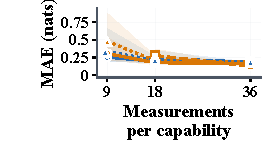
\includegraphics[width=\linewidth]{figs/eff_a.pdf}\caption{Pythia, error against budget}\end{subfigure}\hfill
\begin{subfigure}[t]{1.8in}\centering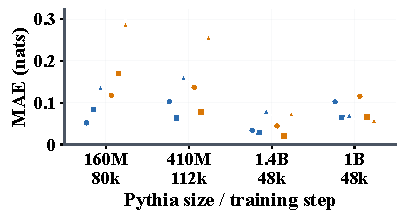
\includegraphics[width=\linewidth]{figs/eff_b.pdf}\caption{OLMo-2, half against full grid}\end{subfigure}\hfill
\begin{subfigure}[t]{1.8in}\centering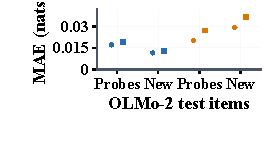
\includegraphics[width=\linewidth]{figs/eff_c.pdf}\caption{Cost of the reduced grid}\end{subfigure}
\caption{Measurement efficiency of the compact pruning form, in nats per native token, on mathematics
and code: error on new Pythia states against development measurements per capability; on the four
OLMo-2 test states, the form fitted on 12 configurations (circles) against the per-density regression
fitted on 24 (squares), on the probes and on the new items; and the recorded cost of the reduced grid
as a share of the full grid, with dense anchors and model loading included.}
\label{fig:efficiency}
\end{figure}

\subsection{Prediction at Unseen Configurations}
\label{sec:unseen_settings}

In grouped quantization, with 54 development and 21 pre-specified test cells, the piecewise
interpolation is the most accurate predictor of unseen group sizes at the development states for
mathematics and code. For distillation, at six new pools and three new budgets, every selected form
improves on zero change, with a detected gain over the development baseline for code on both
students and for question answering on the smaller one.

\subsection{Transfer across Model States}
\label{sec:unseen_states}

On three Pythia checkpoints that entered no fit,
the pre-specified pruning power form matches the per-density regression on mathematics with a quarter of
the parameters, and is less accurate than the median on code and than every source-free curve on
question answering; outside the tested density range every source-conditioned form errs by 0.6 to
4.5 nats. At 2.8B and 6.9B models, beyond the development range, the pre-specified median curve is the more accurate predictor for pruning and per-bit quantization alike, and on a new grouped quantization state it wins for mathematics and question answering, the interpolation for code.



